\section{議論}

\subsection{本手法の有用性}

パソコンやスマートフォンで利用されている様々なテキスト入力システムは
変換方式も使い勝手も全く異なっているのが普通になっているが、
POBox\cite{Masui:POBox}のような単純で柔軟な入力方式を利用すると、
パソコンでもスマートフォンでもほぼ共通の入力を行なうことが可能である。
Gyaimはこのような思想にもとづいて作成されたIMEであるが、
{\system}
あらゆる機器において入力も編集もユニバーサルにすることが可能であろう。

\subsection{本手法の展望}

本論文ではテキストエディタに絞った説明を行なったが、IME はユーザ
のすべてのキー入力を直接受け取る窓口になっているため、編集と関係無いキー操作も IME に担当させることによってより幅広い計算機操作を実行することが
できる。たとえばシステム音量や画面の明るさをコントロールするにはシステ
ムに用意された特別のキーを使ったり、システムに用意されたショートカット
を利用したりすることが多いが、このようなものも IME から制御するようにし
ておけばシステム全体のショートカット設定などは不要になる。


また、文書の整形以外にも、IMEの実装によりテキスト入力を補助するという考え方はより広範な入力に当てはめることができる。
{\system}では、単語の言い換えを補助するために、図\ref{synonym}のように類語を入力することが出来る。

\begin{figure}[H]
\centerline{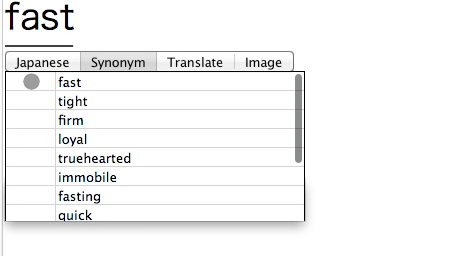
\includegraphics[width=70mm,bb=0 0 350 250]{figures/synonym.png}}
\caption{{\system}の類語変換機能の例。}
\label{synonym}
\end{figure}

図\ref{image1},\ref{image2}は{\system}の画像入力の例である。
ここでは、「知らない」という入力語句について画像を検索し、入力候補として表示している。
画像が埋め込めるテキストエリアであれば画像を埋め込み、そうでなければURLを入力する、といった機能も、IMEにより実装することができる。

\begin{figure}[H]
\centerline{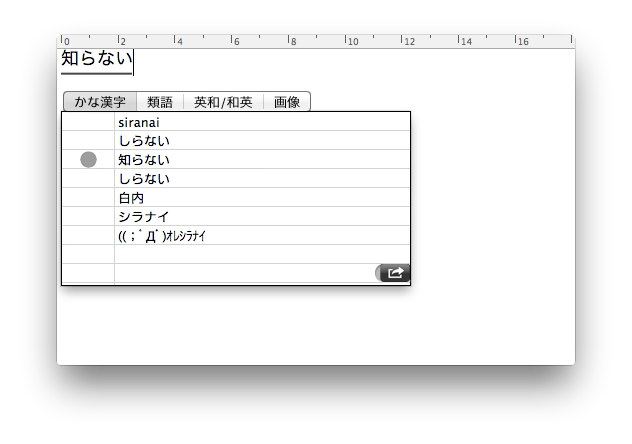
\includegraphics[width=70mm,bb=0 0 600 400]{figures/image1.png}}
\caption{{\system}で「知らない」という単語を入力した例。}
\label{image1}
\end{figure}

\begin{figure}[H]
\centerline{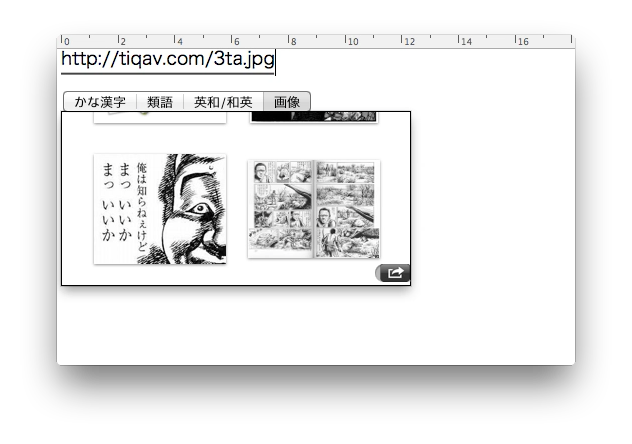
\includegraphics[width=70mm,bb=0 0 600 400]{figures/image2.png}}
\caption{{\system}の画像入力ウィンドウ。}
\label{image2}
\end{figure}

\subsection{本手法の限界}

IME はアプリケーションと独立に実装されているため、
現在のような実装ではアプリケーションの内部状態によって動作を変えたり、
アプリケーションの振る舞いを制御したりすることはできず、表に出ているテキストの編集操作しか
できない。 既存のシステム自体は変更せずに、皮をかぶせる形で機能を拡張す
る手法はある程度有用ではあるが、問題の根本的な解決が必要な場合には限界
がある。テキスト編集の場合は根本的に解決しなければならない問題は多くな
いので、本論文の手法はとりあえず有効だといえるが、根本的な解決のために
は、テキスト入力の枠組みであるIMEに加えて、各コンピュータがテキスト編集
のための枠組みを用意する必要があるだろう。

\subsection{コピー/ペーストと標準化}

Xerox PARCのLarry Teslerが70年代に発明した\cite{Tesler:CopyPaste}
「コピー/ペースト」は現在非常に普及しており、
ほぼすべてのアプリケーションにおいて同じ操作\footnote{
  Macの場合はCommand-CとCommand-V
}でテキストをコピーしたりペーストしたりできるようになっている。
つまりコピー/ペーストに関しては???章で述べたような問題がほぼ存在せず、
ユーザは混乱せずに様々なアプリケーション上でテキスト操作を行なうことが可能になっていることになる。
コピー/ペーストが標準化されているのに対し、
テキスト移動のような処理が全く標準化されていないのは不思議であるし、
そのことに不満を持っているユーザが多くないことも不思議である。
{\system}のような手法を利用することにより、
システム全体を統一的に利用できるようにする工夫が重用であろう。



